\documentclass{beamer}
 
\usepackage[utf8]{inputenc}
\usepackage{hyperref}
\usetheme{Madrid}
\usecolortheme{beaver}
\graphicspath{ {./img/} }

\title{Recursion and Dynamic Programming}
\subtitle{People often joke that in order to understand recursion, you must first understand recursion}
\author[Carocari, Fabris, Lotito]
{Giulia Carocari, Giacomo Fabris, Francesco Lotito}
\institute[UniTN]{Università degli Studi di Trento}
\date[April 10, 2019]
{ICPC Training @ UniTN\\ Day 5 - April 10, 2019}
 
 
 
\begin{document}
 
  \frame{\titlepage}
  \begin{frame} 
      \frametitle{Table of Contents}
      \tableofcontents
  \end{frame}
  \AtBeginSection[]
  {
    \begin{frame}
      \frametitle{Table of Contents}
      \tableofcontents[currentsection]
    \end{frame}
  }
  
  \section{Solutions from last week's contest}
  
  \begin{frame}{A - Almost Union Find}
  \begin{block}{Technique}
  Well...guess what.\\
  Problem applying straightforward UFDS: the "move" operation.
  \end{block}
  
  \begin{block}{Suggestions}
  \begin{itemize}
  \item We can easily move elements from one DS to another if they are leaves
  \item Things get messy if we need to move an internal node
  \item Note: if an element of the set is a leaf, it will continue to be a leaf no matter how many merge operations we invoke.
  \end{itemize}
  \end{block}
  \end{frame}
  
  \begin{frame}{A - Almost Union Find}
  \begin{block}{Solution}
  \begin{description}
  \item[Initialization:] Make the set $S[i]$ be a child of $S[n+i]$
  \item[Move \texttt{(p, q)}:] Find roots: \texttt{x = find(p); y = find(q)}\\
  Then, set \texttt{root[p] = y}.\\ Note that p, q will always be leaves.
  \item[Union:] No change needed.
  \end{description}
  \end{block}
  
  \begin{block}{Note}
  Declare a FT of 64 bit integers (perhaps 32 bit unsigned could have been enough). 
  \end{block}
  \end{frame}
  
  \begin{frame}{B - 10 kinds of people}
  \begin{block}{Technique}
  Seems like flood fill / find connected components. A BFS/DFS will probably result in TLE.\\
  Use Union Find.
  \end{block}
  
  \begin{block}{Solution}
  \begin{itemize}
  \item Each cell of the matrix belongs to one and only one set.
  \item Merge connected sets.
  \item Find roots of queries' elements. If the root is the same, solution may be \texttt{decimal} or \texttt{binary}. Otherwise is \texttt{neither}
  \end{itemize}
  \end{block}
  \end{frame}
  
  \begin{frame}{C - Guess the Data Structure}
  \begin{block}{Technique}
  Simulation
  \end{block}
  
  \begin{block}{Solution}
  \begin{itemize}
  \item Create a stack, a queue, a pqueue.
  \item Insertion: operate insertions on all containers.
  \item Extraction: extract from all containers, compare result with input.
  \end{itemize}
  \end{block}
  \end{frame}
  
  \begin{frame}{D - Fenwick Tree}
  \begin{block}{Technique}
  Fenwick Tree - Range Sum, Point Update
  \end{block}
  
  \begin{block}{Solution}
  \begin{itemize}
  \item See last week's slides
  \item Use 64 bit integers
  \item Heavy I/O, use \texttt{stdio.h}
  \end{itemize}
  \end{block}
  \end{frame}
  
  
  \section{Introduction}
  \begin{frame}
  \frametitle{Introduction}
    \begin{block}{Notes}
        \begin{itemize}
            \item{No Kattis contest today} (yeah, I know you love me)
            \item{Small amount of theory today} (You're loving me even more)
            \item{We will solve some random problems together}
            \item{I'm planning to publish some notes on Dynamic Programming on \url{https://www.fralotito.me}}
        \end{itemize}
    \end{block}
    
    \pause

    \alert{You need to have an account on} 
    \begin{itemize}
      \item{AtCoder} \url{https://atcoder.jp/}
      \item{Kattis} \url{https://open.kattis.com/}
    \end{itemize}
  \end{frame}
  
  \section{Divide and conquer / Divide et Impera}

  \begin{frame}{Divide et whaaat?}
    \begin{block}{Let's Google it}
      \textit{"A divide-and-conquer algorithm works by recursively breaking down a problem into two or more sub-problems of the same or related type, until these become simple enough to be solved directly. The solutions to the sub-problems are then combined to give a solution to the original problem."}
    \end{block}
  \end{frame}

  \begin{frame}{Some examples}
    \begin{itemize}
      \item \href{https://www.geeksforgeeks.org/python-program-for-binary-search/}{Binary search}
      \item \href{https://www.geeksforgeeks.org/euclidean-algorithms-basic-and-extended/}{Euclidean Algorithm (GCD)}
      \item \href{https://www.geeksforgeeks.org/merge-sort/}{Merge sort / Quick sort}
      \item \href{https://www.geeksforgeeks.org/fast-fourier-transformation-poynomial-multiplication/}{Fast Fourier Transform}
    \end{itemize}
    
    \pause
    \alert{Note:} You can click on them and get a tutorial
  \end{frame}
  
  \section{Fibonacci}
  \begin{frame}{Fibonacci}
    \begin{block}{Problem definition}
        The Fibonacci numbers are the numbers in the following integer sequence: \newline
        $0, 1, 1, 2, 3, 5, 8, 13, 21, 34, 55, 89, 144, ..$

        In mathematical terms, the sequence $F_n$ of Fibonacci numbers is defined by the recurrence relation: \newline
        \begin{equation}
            F(n)=\begin{cases}
            0 & \text{if $n=0$}.\\
            1 & \text{if $n=1$}. \\
            F(n-1) + F(n-2) & \text{otherwise}.
            \end{cases}
        \end{equation}
        \newline
        Print the n-th Fibonacci Number.
    \end{block}
    \pause
    \setbeamercolor{block title}{use=structure,fg=white,bg=cyan!75!black}
    \begin{block}{Solution}
    Well.. there are lots of them :)
    \end{block}
  \end{frame}
  
  \begin{frame}{Fibonacci}
    \setbeamercolor{block title}{use=structure,fg=white,bg=cyan!75!black}
    \begin{block}{Solution}
        \begin{itemize}
            \item Use recursion: exponential
        \end{itemize}
    \end{block}
    \pause
    \begin{center}
        After one day of computation..
        
\includegraphics[scale=0.35]{shit}
    \end{center}
  \end{frame}
  
    \begin{frame}{Fibonacci}
    \setbeamercolor{block title}{use=structure,fg=white,bg=cyan!75!black}
    \begin{block}{Let's make Fibonacci great again}
        \begin{itemize}
            \item Add memoization (DP): $O(n) time, space$
            \pause
            \item Bottom-up (DP): $O(n) time, space$
            \pause 
            \item Bottom-up + space optimization (DP): $O(n) time, O(1) space$
            \pause
            \item Closed formula: $O(1) time, space$
            $$f(n) = \frac{1}{\sqrt{5}}\left[\left(\frac{1+\sqrt{5}}{2}\right)^{n+1}-\left(\frac{1-\sqrt{5}}{2}\right)^{n+1}\right]$$
        \end{itemize}
    \end{block}
  \end{frame}
  
  \begin{frame}{Why does DP work?}
    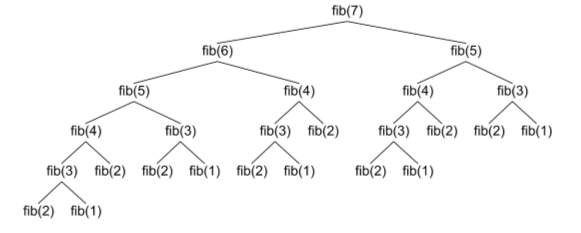
\includegraphics[scale=0.8]{fib}
  \end{frame}
  
  \begin{frame}{Unlimited power}
    
\includegraphics[scale=0.65]{meme1}
  \end{frame}

  
  \section{Dynamic Programming}
  \begin{frame}
  \frametitle{Dynamic Programming}
    \begin{block}{Idea}
    The idea is very simple, if you have solved a problem with the given input, then save the result for future reference, so as to avoid solving the same problem again.. shortly ‘Remember your Past’
    \end{block}
  \end{frame}
  
  \begin{frame}
  \frametitle{Dynamic Programming}
    \begin{block}{Top-down vs Bottom up}
    \begin{itemize}
        \item If all subproblems must be solved at least once, a bottom-up dynamic-programming algorithm usually outperforms a top-down memoized algorithm by a constant factor.
        \begin{itemize}
            \item No overhead for recursion and less overhead for maintaining table.
            \item There are some problems for which the regular pattern of table accesses in the dynamic-programming algorithm can be exploited to reduce the time or space requirements even further.
        \end{itemize}
        \item If some subproblems in the subproblem space need not be solved at all, the memoized solution has the advantage of solving only those subproblems that are definitely required.

    \end{itemize}
    \end{block}
  \end{frame}
    
    \begin{frame}
    \frametitle{Dynamic Programming}
      \begin{huge}
        \begin{center}
          Educational DP contest: problems A to G, \textbf{NO E}
        \end{center}
      \end{huge}
    \end{frame}
    
    

\end{document}
